%% jdavid-jdecker-nb-text-classifier.tex
%% Jon David and Jarrett Decker
%% March 2016
%%
%%-------------------------------------------------------------------
%% Notes to self:
%%
%% Package algpseudocode and algorithm need to be installed. Try:
%%   sudo apt-get install texlive-science
%%
%% Adding graphics to LaTeX document:
%%   https://www.sharelatex.com/learn/Inserting_Images


\documentclass{IEEEtran}

\usepackage[style=ieee,backend=bibtex]{biblatex}
\usepackage{hyperref}
\usepackage{amsmath}
\usepackage{algpseudocode}
\usepackage{algorithm}
\usepackage{graphicx}
%%\usepackage{appendix}

%% Tell LaTeX where the images are located
\graphicspath{ {figures/} }

\hypersetup{hidelinks}

%%% ADD RELEVANT REFERENCES HERE %%%
%\addbibresource{quinlan1986.bib}
%\addbibresource{schlimmer1981.bib}
\addbibresource{mitchell1997.bib}
\addbibresource{yang1999.bib}



\author{Jarrett Decker*\thanks{e-mail:
    \href{mailto:jdeck069@unm.edu}
         {\texttt{jdeck069@unm.edu}}
         {*authors contributed equally}} and
\and
       Jon David*\thanks{e-mail:
    \href{mailto:jdavid@cs.unm.edu}
         {\texttt{jdavid@cs.unm.edu}}
         {*authors contributed equally}}}

\title{An Implementation of a Naive Bayes Classifier on Text Classification}

\begin{document}

\maketitle

\begin{abstract}
This report describes how we trained a Naive Bayes classifier to classify words in newsgroup articles, experiments over various settings, and results. We also discuss some natural questions that arise from such experiments.
\end{abstract}


\section{Introduction}
Naïve Bayes classifiers are a powerful, yet relatively simple, method of doing classification. By leveraging Bayes theorem, the difficult problem of predicting a class based off of a group of attributes can be transformed into the easier task of estimating the chance of those attributes appearing, given a specific class. This is the heart of the Naïve Bayes classification algorithm.

Compared to humans, computers can parse documents incredibly fast, but knowing what the documents are about has traditionally been something only humans can do reliably. With the progress made in machine learning computers can now classify documents at reasonable accuracies. The task of this project was to classify documents into one of twenty “newsgroups” using a Naïve Bayes classifier. Our model did not take word position into account and treated documents as a “bag of words”. 

Naïve Bayes is a good choice for this type of problem because the simplicity of classification allows us to easily handle large data sets, such as all words in the English language.  Naïve Bayes classifiers can also be tweaked through changing beta values in the MAP estimation, or manipulating the data set through things like deleting certain stop words, which could confuse the classifier. This allows you the flexibility to tune your classifier to your problem, making this algorithm useful for many applications, including document classification.

\section{Design and Implementation}
The main features of the Naïve Bayes classifier are the MLE, MAP, and classification functions. Our design modularized these functions through object oriented programming methods, as well as utility functions. 

\subsection{Data Structures}
Our data necessitated the use of python’s numpy arrays to represent our calculated probabilities. By representing our data in this way, the classification function became a simple addition and matrix multiplication. Along with numpy arrays we also saved our MLE and MAP values to .model files, so we could capture these values and not have to retrain the system every time a classification was run.

\subsection{Naive Bayes Training}

Our design implemented a Trainer class that was in charge of reading in the data and labels and then creating the MLE and MAP models that our classifier uses. This class only has to train once to create the model files and those files are available for classification without having to be retrained. 

The first function of training is to calculate the MLE of the training labels. The purpose of this is to determine the probability of any label appearing for an unknown document. This probability has nothing to do with what words are associated with what labels, just the rate at which labels appear in the training set. The MLE equation is defined in \ref{eq:mle}

\begin{equation}
\label{eq:mle}
P(Y_k) = \dfrac{number.of.documents.labeled. Y_k}{total.number.of.documents}
\end{equation}

The second function of training is to determine the MAP of the attributes of the training set. The MAP function allows you to adjust your results to either more resemble what you found in the training set, or to a prior estimation that you can set through the beta value. This beta value is very important, it makes it possible to classify with attributes that you may not have seen for any class before. Usually if you see an attribute that has never been seen belonging to a class, the probability of the unknown class equaling that class will now be zero, but by using the prior beta value instead of zeroing out the probability you can just set it to something small. Since chances are high that classifying combinations of attributes that were not present in the training set, having a beta protects you from having a classification saying there is a zero percent chance of the attributes belonging to any class.

The MAP equation is defined in Figure \ref{eq:map}.

\begin{equation}
\label{eq:map}
P(X_i|Y_k) = \dfrac{(count.of. X_i .in. Y_k) + (\alpha-1)}{(words.in. Y_k) + ((\alpha-1)(length.of.vocab))}
\end{equation}

Where $\alpha=1+\beta$.

\subsection{Naive Bayes Classification}
We implemented a NaiveBayesClassifier class that was able to use the MLE and MAP from the trainer to do the calculations needed to classify new data. The classifier writes its classifications to a text file in order to be compared to the truth data for the determination of accuracy. We use Equation \ref{eq:classify} to classify words as belonging to one of the newsgroups.

\begin{equation}
\label{eq:classify}
Y_{new} = argmax(log_2(\overrightarrow{a}) + \overrightarrow{b} \times log_2(C))
\end{equation}

Where $\overrightarrow{a}$ is an MLE vector, $\overrightarrow{b}$ is a vector of new words to classify, and $C$ is a matrix produced by calculating MAP over the set of pairs of all words and newsgroups.


\subsection{Confuion Matrix and Accuracy}
A confusion matrix is useful for visualizing the results of classification. Accuracy can also be determined from the confusion matrix. We created a ConfusionMatrix class that can read the predicted values that the classifier determined, and the true values from the data set and then increments an element in the confusion matrix associated with those values. For example, if the predicted label was 4 and the true label was 5, the element indexed by [4][5] would be incremented. It follows that elements lying along the diagonal are all accurate predictions while elements off of the diagonal are incorrect. By totaling the values along the diagonal and dividing by the sum of all the values in the matrix the total accuracy of the predictions can be found. 

\subsection{Utility Clases}
To help with the other parts of the program, we added some utility classes. The Vocabulary class was used to store all possible words in our vocabulary and was capable of producing words associated with word IDs and vice versa. The NewsGroups class was similar, except instead of storing information about the words, it stored information about the possible labels, including the size of the set of labels and the names and IDs.

\section{Experiments}
\subsection{Data}
To classify text documents, both training and test files are provided. Definition files are also provided.

\subsubsection{Definition Files}
The vocabulary.txt is a definition file that defines that set of all words that appear in the data set. It is a simple text file where each line represents a word, whose word ID is the line number in that file. The newsgroups.txt file is a definition file that defines the set of all news groups that appear in the data set. It is a simple text file where each line represents a news group, whose news group ID is the line number in that file.

\subsubsection{Data Files}
There are two data files: train.data, and test.data. The train.data file is used for training the model and the test.data file is used to evaluate the performance and accuracy of the model. Both files have the same format. These are text files where each line consists of a document ID, word ID, and word count. Each line represents the number of instances a particular word appears in a particular document. This means the word counts for each word in a document are distributed throughout multiple lines.

\subsubsection{Label Files}
There are two label files: train.label, and test.label. The train.label file is used for training the model and the test.data file is used to evaluate the performance accuracy of the model. Both files have the same format. These are text files where each line consists of a single integer representing a newsgroup ID. The line number represents the document ID. The file is a mapping between document IDs and news group IDs. For each line, the document is classified as a type of news group.


\subsection{Methods}
Naive Bayes classifiers are built by calculating the maximum likelihood estimate (MLE), and the maximum a priori (MAP). This calculation is described in the implementation section. This experiment builds several naive bayes classifier models with various settings: (1) various beta-value in the range [0.00001, 1.0], and (2) stop-word inclusion or exclusion. [Hmm include a sentence that explains what the beta-value is and what it's for?]

Ten models of various beta values are generated and their performance is compared against each other. Two models using the same beta value, but differing only in the inclusion or exclusion of stop-words, are also generated and compared against each other.

\subsection{Results}
\subsubsection{The effects of various beta-values}

\begin{figure}
  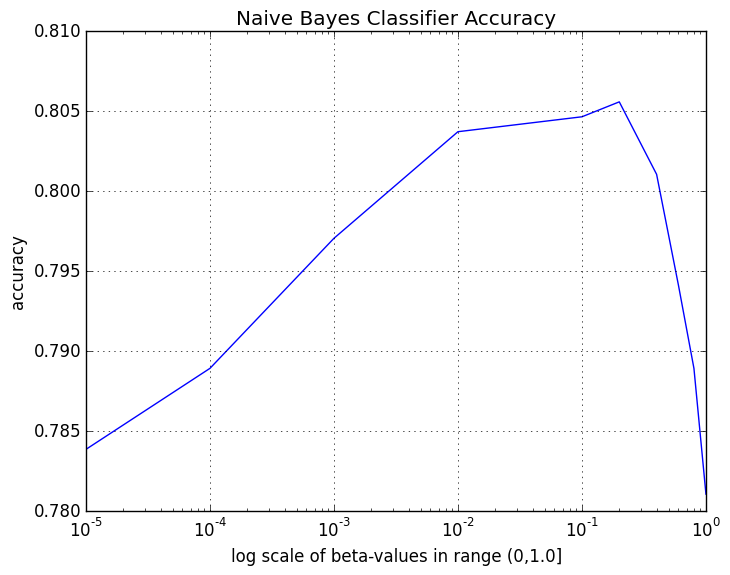
\includegraphics[width=0.4\textwidth, natwidth=80,natheight=80]{betavsacc.png}
  \caption{Performance of classifier with different beta-values}
  \label{fig:betavsacc}
\end{figure}

Figure \ref{fig:betavsacc} shows performance of Naive Bayes Classifier over different values of beta. For small values of beta (0.00001), the accuracy is less than .785. As beta values increase, accuracy increases until reaching beta value of around 0.1. At beta value 0.1, accuracy peaks at 0.80. From this point, any increase in beta rapidly decreases accuracy. At beta value of 1.0, accuracy drops below 0.785.

This behavior may be explained by analyzing $\beta$'s rule in Equation \ref{eq:map}, the MAP equation. Looking at the $\beta$-value in the MAP equation, we can see that for small counts of $X_i$, $\beta$ becomes significant. For small counts of $X_i$, if we decrease $\beta$ the numerator becomes very small, as seen in Figure \ref{fig:betavsacc}. Similarly, when $\beta$ approaches 1.0, $\beta$ plays a larger role in the denominator. This is because as $\beta$ increases, the denominator increases more rapidly than the numerator. When the denominator is much larger than the numerator, result is a very small number. As seen in Figure \ref{fig:betavsacc}, when $\beta$ approaches 1.0 accuracy drops significantly.

\subsubsection{The effects of English stop-words}
Two models with the same beta-value are also compared. One model diminishes the weight of English stop-words, and the other treats English stop-words the same as every other word in the vocabulary. The model that diminishes the weight of English stop-words produces an accuracy of 0.80 over the test set. The other model produces an accuracy of 0.78 over the test set. [So what? what is the significance of that?]

\begin{table}[ht]
  \caption{Comparing effects of English stop-words on accuracy}
  \centering
  \begin{tabular}{c c c }
  \hline\hline
           & Model A & Model B \\ [0.5ex]
  %heading
  \hline
  Accuracy &   0.785 &   0.800 \\ [1ex]
  \hline
  \end{tabular}
  \label{table:stopwords}
\end{table}

Table \ref{table:stopwords} compares the results of two models. Call these models Model A and Model B. Model A treats English stop-words as all of the other words. Model B reduces the weight of English stop-words. The latter has slightly higher accuracies.

\section{Discussion}

%% Question 1 %%%%%%%%%%%%%%%%%%%%%%%%%%%%%%%%%%%%%%%%%%%%%%%%%%%%%%%
\subsection{Explain why it would be difficult to accurately estimate the parameters of this model on a reasonable set of documents.}
The model given is:

\begin{equation}
\label{entropy-equation}
(P(Y|X_{1..d}) \propto P(X_{1..d}|Y)*P(Y) = P(Y)*\prod(P(X_i|Y))
\end{equation}

It would be difficult to accurately estimate the parameters of this model on a reasonable set of documents because there are too many (how many?) parameters. For larget data sets estimating the parameters of this model becomes intractable.
Answers go here.


% %% Question 2 %%%%%%%%%%%%%%%%%%%%%%%%%%%%%%%%%%%%%%%%%%%%%%%%%%%%%
\subsection{Report your overall testing accuracy and print out the confusion matrix}
The accuracy for our model with beta-value $\dfrac{1}{size(V)}$ is 0.785. This confusion matrix can be found in Table \ref{table:confmatrix} in Appendix II. It is in the Appendix because the table is too large to fit in a two-column page.


%% Question 3 %%%%%%%%%%%%%%%%%%%%%%%%%%%%%%%%%%%%%%%%%%%%%%%%%%%%%%%
\subsection{Are there any newsgroups that the algorithm confuses more ofthen than others? Why do you think this?}

Table \ref{table:confmatrix} is the confusion matrix produced for generated model with beta-value 0.1, excluding stop-words. The confusion matrix is a useful tool to help visualize what types of errors occur in the model. The confusion matrix's two axis are the predicted labels(columns), and actual labels(rows). The number in each cell[x][y] represents the number of times a prediction y was made when the true value was x. The main diagonal represents the correct prediction. All other values outside the main diagonal represent incorrect prediction.

Because of the confusion matrix, we can easily answer this question. Yes, there are more than a few newsgroups that the algorithm confuses more often than others. Some examples are confusion between the newsgroups: (1) predicted alt.atheism vs talk.religion.misc; (2) comp.graphics vs comp.os.ms-windows.misc; (3) comp.os.ms-windows.misc vs comp.sys.ibm.pc.hardware; (4) comp.graphics vs comp.windows.x; (5) sci.electronics vs comp.sys.ibm.pc.hardware.

It's very likely that the algorithm got confused because these pairs of newsgroups are similar because they share common vocabulary. As in the examples given above, alt.atheism and talk.religion.misc talk about religion; sci.electronics vs comp.sys.ibm.pc.hardware talk about PC hardware which is a type of electronics device; comp.graphics and comp.windows.x talk about things displayed on the screen; etc.


%% Question 4
\subsection{Retrain your Naive Bayes classifier for values of beta between 0.00001 and 1 and report the accuracy over the test set for each value of B. Create a plot with values of beta on the x-axis and accuracy on the y-axis. Use a logarithmic scale for the x-axis. Explain in a few sentences why accuracy drops for both small and large values of beta.}
The naive bayes classifier models with beta-values ranging from 0.00001 and 1.0 produce accuracies, over the test set, shown in Figure \ref{fig:betavsacc}.

Figure \ref{fig:betavsacc} shows performance of Naive Bayes Classifier over different values of beta. For small values of beta (0.00001), the accuracy is less than .785. As beta values increase, accuracy increases until reaching beta value of around 0.1. At beta value 0.1, accuracy peaks at 0.80. From this point, any increase in beta rapidly decreases accuracy. At beta value of 1.0, accuracy drops below 0.785.


This behavior may be explained by analyzing $\beta$'s rule in Equation \ref{eq:map}, the MAP equation. Looking at the $\beta$-value in the MAP equation, we can see that for small counts of $X_i$, $\beta$ becomes significant. For small counts of $X_i$, if we decrease $\beta$ the numerator becomes very small, as seen in Figure \ref{fig:betavsacc}. Similarly, when $\beta$ approaches 1.0, $\beta$ plays a larger role in the denominator. This is because as $\beta$ increases, the denominator increases more rapidly than the numerator. When the denominator is much larger than the numerator, result is a very small number. As seen in Figure \ref{fig:betavsacc}, when $\beta$ approaches 1.0 accuracy drops significantly.

%% Question 5
\subsection{Propose a method for ranking the words in the dataset based on how much the classifier 'relies on' them when performing its classification. It should give high schores to those words that appear frequently in one or a few of the newsgroups but not in other ones. Words that are used frequently in general English should have lower scores, as well as words that only appear extremely rarely throughout the whole dataset.}

In \parencite{yang1997comparative}, Yang compares several methods on feature selection in text configuration. We use one of his methods for word ranking. In text classification, information gain is a natural way to perform feature selection. Using only our MLE and MAP values we were able to implement the information gain formula. Equation \ref{eq:infogain} can be found in Appendix D. It is too long to fit in two a two column page.

For info gain as well as the equations saying P(X,Y) = P(X|Y)P(Y), P(X) = sum over Y(P(X,Y)), and that MAP = P(X|Y), MLE = P(Y)

By applying this to our vocabulary we were able to get information gain values for every word. We then removed certain “stop words” by setting those words information gain to 0. If we didn’t do this, there were a number of words that occur regularly in all documents, such as “a” and “the” that appears to be a top word. After removing those words the top k values could then be found and listed as a ranked list of words.


%% Question 6
\subsection{Implement your method, set beta back to $\dfrac{1}{V}$ and print out the 100 words with the highest measure.}
The Top 100 words can be found in Appendix C at the end of this document. But the top ten are windows, god, scsi, car, drive, space, team, dos, bike, file. But for the full 100 go to Appendix C.

%% Question 7
\subsection{If the points in the training dataset were not sampled independently at random from the same distribution of data we plan to classify in the future, we might call that training set biased. Dataset bias is a problem because the performance of a classifier on a biased dataset will not accurately reflect its future performance in the real world. Look again at the words your classifier is 'relying on'. Do you see any signs of dataset bias?}
A number of the religious words in the top 100 list appear to be biased towards western religions. Christ, Jesus, Jew, bible, and Christians, all appear on the list, but other religions terms do not. This is possibly because most English speaking countries are either Christian or Jewish majorities. It might be difficult for this classifier to classify documents about other, non-western, types of religions. The solution to these types of data set problems is usually to gather more data from the space that you’re trying to classify in.
  


\printbibliography

\newpage
\onecolumn
\appendix
\section{Appendices}
\subsection{Confusion Matrix}
A confusion matrix is more descriptive of a model's performance than accuracy. A confusion matrix shows the number of true positives (TP), true negatives (TN), false positives (FP), and false negatives (FN). From this accuracy and misclassification can be calculated. Accuracy is (TP+TN/p+e) and Misclassification is 1.0-Accuracy.

\begin{table}[ht]
  \caption{Confusion Matrix}
  \centering
  \begin{tabular}{c c c c c c c c c c c c c c c c c c c c c}
   \hline\hline
       &  1 &   2 &   3 &   4 &   5 &   6 &   7 &   8 &   9 &  10 &  11 &  12 &  13 &  14 &  15 &  16 &  17 &  18 &  19 &  20 \\
   %heading
   \hline
     1 & 247 &   0 &   0 &   0  & 0 &  1 & 0 & 0 & 2 & 0 & 0 &  2 & 0 & 3 &  6 & 23 & 2 & 3 & 4 & 25 \\
     2 &   0 & 290 &  14 &  15  & 8 & 21 & 6 & 0 & 0 & 0 & 1 & 10 & 8 & 4 & 11 &  1 & 0 & 0 & 0 &  0 \\
     3 &   1 &  35 & 212 &  55  &16&21&6&2&3&0&0&8&3&11&10&1&2&0&3&2 \\
     4 &   0 &  12 &  34 & 271 &16&2&16&2&0&0&1&3&32&1&2&0&0&0&0&0 \\
     5 &   0 &  21 &  11 &  32 &261&2&17&1&2&0&0&3&19&8&5&0&1&0&0&0 \\
     6 &   0 &  54 &  15 &   5 &3&291&1&1&2&0&0&4&2&6&4&0&1&0&1&0 \\
     7 &   0 &   7 &   5 &  30 &12&1&279&15&10&1&2&0&7&4&6&0&1&0&1&1 \\
     8 &   0 &   3 &   1 &   2 &0&0&17&330&19&0&0&1&12&0&4&1&0&0&4&1 \\
     9 &   0 &   1 &   0 &   1 &0&0&2&24&363&0&0&0&3&1&0&0&1&1&0&0 \\
    10 &   0 &   0 &   1 &   1 &0&0&3&1&1&355&18&0&1&3&5&2&1&0&4&1 \\
    11 &   1 &   0 &   1 &   0 &0&0&2&0&2&3&385&1&0&1&0&1&1&0&1&0 \\
    12 &   0 &   3 &   1 &   3 &3&1&1&0&0&0&1&361&3&2&3&0&10&0&3&0 \\
    13 &   3 &  24 &   5 &  25 &6&3&12&9&6&0&1&20&257&10&9&0&3&0&0&0 \\
    14 &   2 &   7 &   0 &   3 &0&0&4&5&1&2&1&1&9&328&10&5&6&3&5&1 \\
    15 &   0 &   9 &   0 &   1 &0&5&1&0&1&0&1&4&6&6&346&1&2&1&8&0 \\
    16 &  11 &   2 &   0 &   0 &0&2&1&0&0&0&0&0&0&3&2&356&1&1&1&18 \\
    17 &   1 &   1 &   0 &   0 &0&1&1&2&1&1&0&4&0&6&2&1&307&4&21&11 \\
    18 &  11 &   1 &   0 &   2 &0&0&0&2&0&2&0&2&1&0&0&5&3&327&20&0 \\
    19 &   6 &   1 &   0 &   0 &1&1&0&1&0&0&0&6&1&12&6&2&62&5&193&13 \\
    20 &  36 &   4 &   0 &   0 &0&0&0&0&1&1&0&1&0&5&6&22&11&4&10&150 \\
    \hline
  \end{tabular}
  \label{table:confmatrix}
\end{table}

\subsection{Newsgroup IDs}

\begin{table}[ht]
  \caption{Newsgroup IDs}
  \centering
  \begin{tabular}{c c }
  \hline\hline
  ID & Newsgroup (ID) \\ [0.5ex]
  %heading
  \hline
   1 & alt.atheism \\
   2 & comp.graphics \\
   3 & comp.os.ms-windows.misc \\
   4 & comp.sys.ibm.pc.hardware \\
   5 & comp.sys.mac.hardware \\
   6 & comp.windows.x \\
   7 & misc.forsale \\
   8 & rec.autos \\
   9 & rec.motorcycles \\
  10 & rec.sport.baseball \\
  11 & rec.sport.hockey \\
  12 & sci.crypt \\
  13 & sci.electronics \\
  14 & sci.med \\
  15 & sci.space \\
  16 & soc.religion.christian \\
  17 & talk.politics.guns \\
  18 & talk.politics.mideast \\
  19 & talk.politics.misc \\
  20 & talk.religion.misc \\

  \hline
  \end{tabular}
  \label{table:newsgroupids}
\end{table}


\subsection{Top 100 Words}
\textbf{Top 100 Words:}
  windows,
  god,
  scsi,
  car,
  drive,
  space,
  team,
  dos,
  bike,
  file,
  mb,
  game,
  key,
  mac,
  jesus,
  window,
  dod,
  hockey,
  graphics,
  card,
  image,
  gun,
  encryption,
  sale,
  apple,
  government,
  season,
  games,
  israel,
  disk,
  files,
  ide,
  controller,
  players,
  shipping,
  chip,
  program,
  cars,
  nasa,
  win,
  year,
  turkish,
  motif,
  people,
  armenian,
  play,
  drives,
  bible,
  use,
  widget,
  pc,
  clipper,
  offer,
  jpeg,
  baseball,
  bus,
  nhl,
  software,
  db,
  server,
  jews,
  os,
  israeli,
  output,
  data,
  system,
  league,
  armenians,
  christian,
  christians,
  entry,
  mhz,
  ftp,
  price,
  christ,
  guns,
  thanks,
  church,
  color,
  teams,
  privacy,
  condition,
  launch,
  com,
  monitor,
  ram,
  memory,
  keys,
  display,
  mouse,
  ride,
  using,
  images,
  law,
  video,
  faith,
  computer,
  orbit,
  version,
  mail,

\subsection{Information Gain Equation}
\begin{equation}
\label{eq:infogain}
G(t) = -\sum_{i=1}P(c_i)P(c_i)
+ P(t)\sum_{i=1}P(c_i|t)log P(c_i|t)
+ P(\bar(t))\sum_{i=1}P(c_i|\bar(t))log P(c_i|t)
\end{equation}


\end{document}